\lstset{style=fsharpstyle}

\section{Моделирование предметной области} 
\label{sec:practice:technology_used}


\subsection{Use-case диаграмма }
\label{sub:practice:microsoft_net}

Use-case diagram в UML – диаграмма, отражающая отношения между актёрами и прецедентами и являющаяся составной частью модели прецедентов, позволяющей описать систему на концептуальном уровне.

Прецедент – возможность моделируемой системы (часть её функциональности), благодаря которой пользователь может получить конкретный, измеримый и нужный ему результат. Прецедент соответствует отдельному сервису системы, определяет один из вариантов её использования и описывает типичный способ взаимодействия пользователя с системой. Варианты использования обычно применяются для спецификации внешних требований к системе. Основное назначение диаграммы – описание функциональности и поведения, позволяющее заказчику, конечному пользователю и разработчику совместно обсуждать проектируемую или существующую систему.

При моделировании системы с помощью диаграммы прецедентов системный аналитик стремится:
\begin{itemize}
  \item чётко отделить систему от её окружения;
  \item определить действующих лиц (актёров), их взаимодействие с системой и ожидаемый функционал системы;
  \item определить в глоссарии предметной области понятия, относящиеся к детальному описанию функционала системы (то есть, прецедентов);
\end{itemize}

Работа над диаграммой может начаться с текстового описания, полученного при работе с заказчиком. При этом нефункциональные требования (например, конкретный язык или система программирования) при составлении модели прецедентов опускаются (для них составляется другой документ).
Для отражения модели прецедентов на диаграмме используются:

\begin{itemize}
  \item рамки системы – прямоугольник с названием в верхней части и эллипсами (прецедентами) внутри. Часто может быть опущен без потери полезной информации;
  \item актёр обозначает набор ролей пользователя (понимается в широком смысле: человек, внешняя сущность, класс, другая система), взаимодействующего с некоторой сущностью (системой, подсистемой, классом). Актёры не могут быть связаны друг с другом (за исключением отношений генерализации/наследования);
  \item  прецедент – эллипс с надписью, обозначающий выполняемые системой действия (могут включать возможные варианты), приводящие к наблюдаемым актёрами результатам. Надпись может быть именем или описанием (с точки зрения актёров) того, <<что>> делает система (а не <<как>>);
\end{itemize}

Имя прецедента связано с непрерываемым (атомарным) сценарием – конкретной последовательностью действий, иллюстрирующей поведение. В ходе сценария актёры обмениваются с системой сообщениями. Сценарий  может быть приведён на диаграмме прецедентов в виде UML-комментария. С одним прецедентом может быть связано несколько различных сценариев.

Для представления функциональной модели была выбрана диаграмма вариантов использования - UML, которая отражает отношения между актерами и прецедентами и позволяет описать систему на концептуальном уровне. Прецедент соответствует отдельному сервису системы, определяет один из вариантов её использования и описывает типичный  способо взаимодействия пользователй с системой. UML предназначен для определения, визуализации, проектирования и документирования программных систем.

\begin{figure}[ht]
\centering
  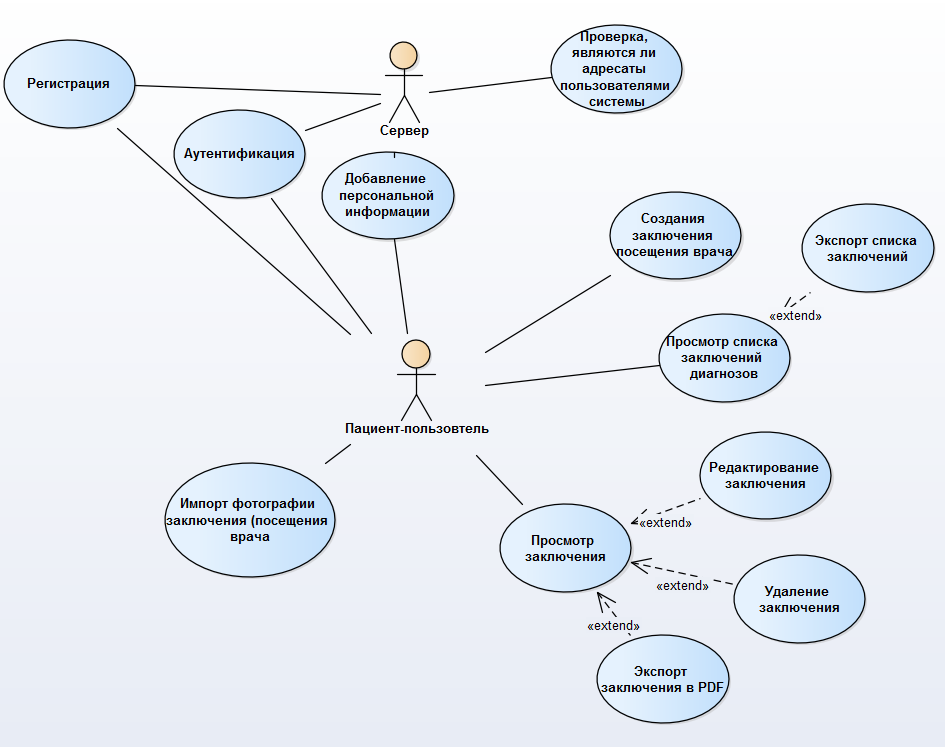
\includegraphics[scale=0.7]{usecase.png}  
  \caption{ Диаграмма вариантов использования. }
  \label{fig:domain:manual_structure:credit_usecase}
\end{figure}


\subsection{Спецификация требований }
\label{sub:practice:tab_task}

Исходя из анализа литературы и аналогов, разработанной схемы базы данных, было разработано техническое задание к мобильному программному средству «Органайзер здоровья пациента»: 

\begin{enumerate}
\item Создание модуля регистрации и авторизации
\item Создание модуля для создания и редактирования персональной информации пользователя
\item Создание модуля создания и редактирования медицинских карточек (заключение посещения врача)
\begin{enumerate}
\item Подключение модуля поиска для эффективного поиска заключений
\item Реализация логики сохранения заключений в БД
\item Реализация логики обновления всех информационных полей заключений
\end{enumerate}
\item Создание модуля работы с медикаментами
\begin{enumerate}
\item Реализация возможности добавления медикаментов
\item Реализация логики сохранения медикаментов в БД
\item Реализация логики создания расписания приема медикаментов
\item Реализация логики управления событиями
\item Реализация возможности установки уведомления о приеме медикаментов по расписанию
\end{enumerate}
\item Создание модуля диагностических заключений
\begin{enumerate}
\item Реализация возможности просмотра списка диагностических заключений
\item Реализация создания и редактирования диагностических заключений
\item Реализация логики сохранения диагностики в БД
\item Подключение модуля поиска для эффективного поиска диагностических заключений
\end{enumerate}
\item Реализация модуля настроек системы
\begin{enumerate}
\item Удаление выборочной информации о карточках пациента
\end{enumerate}
\end{enumerate}
